%#!platex kadai2006_04

\section{$BFsJ,LZ(B}

% \section{$B<BAu$K$*$1$k;EMM(B}
% \label{sec:Specification}

% $B%j%9%H$N35G0$rM}2r$7$F$b(B, $B<B:]$K%W%m%0%i%`$H$7$F<BAu$9$kCJ$K$J$k$H:Y$+(B
% $B$$$H$3$m$^$G7h$a$F$*$/I,MW$,$"$k(B.
% $B%j%9%H$N<BAu$N;EMM$H$7$FMM!9$J$b$N$,9M$($i$l$k$,(B, $BK\<B83$G$O0J2<$K<($9(B
% $B;EMM$r:NMQ$9$k$3$H$K$9$k(B.
% $B$^$?(B, $BFbMF$KJQ99$,$"$k$J$7$K4X$o$i$:(B, $B;EMM$OI,$:%l%]!<%H$K5-=R$9$k$3$H(B.


% \begin{itemize}
% \item $B%;%k%G!<%?$O(B \texttt{int} $B7?$N%G!<%?(B 1 $B8D$@$1$G$"$k(B.
% \item $B<!$N%;%k$,B8:_$7$J$$>l9g$K$O(B, $B<!$N%;%k$X$N%]%$%s%?$r(B
%   \texttt{NULL} $B$H$9$k(B.
%   $B$9$J$o$A(B, $B<!$N%;%k$H$7$F(B \texttt{NULL} $B$rJ];}$9$k%;%k$O(B, $B%j%9%H$N=*(B
%   $BC<$H$J$k(B.
% \item $B%;%k$NA^F~$O(B, $B>l=j$N;XDj$K;HMQ$7$?%;%k$H$=$ND>A0$N%;%k$N4V$KA^F~(B
%   $B$9$k(B.
% \item $B%j%9%H$N@hF,$H$7$F(B, $B%@%_!<$N%;%k$rMQ$$$k(B.
%   $B$9$J$o$A(B, $B%@%_!<%;%k$N<!$N%;%k$,%j%9%H$N@hF,$N%;%k$H$J$k(B.
% \item $B%;%k$N?75,:n@.$K$O(B \texttt{malloc} $B$r;HMQ$7(B, $B:o=|;~$K$O(B
%   \texttt{free} $B$r;HMQ$7$F%a%b%j$rF0E*$K3NJ](B/$B2rJ|$9$k(B.
% \item $BA`:n4X?t$O(B, $B%j%9%H$N?75,:n@.(B (MAKENULL), $B<!$N%;%k(B/$BA0$N%;%k$X$N%](B
%   $B%$%s%?$N<hF@(B (NEXT/PREVIOUS), $B%j%9%H$N@hF,$N%;%k(B/$B=*C<$N%;%k$X$N%]%$(B
%   $B%s%?$N<hF@(B (FIRST/END), $B%;%k$N?75,A^F~(B (INSERT), $B%;%k$N:o=|(B
%   (DELETE), $B%;%k0LCV$N<hF@(B (LOCATE), $B%;%k%G!<%?$N<hF@(B (RETRIVE), $B%j%9(B
%   $B%HFbMF$NI=<((B (PRINTLIST) $B$K%j%9%HA4BN$N:o=|$r2C$($?7W(B 11 $B4X?t$+$i9=(B
%   $B@.$9$k(B.
% \end{itemize}

$B<!2s$N<B83$GMxMQ$7$d$9$$$h$&$K!"9=B$BN@k8@!"4X?t$N%W%m%H%?%$%W@k8@Ey$O(B
$B%X%C%@%U%!%$%k$K!"A`:n4X?t72$HA`:n%W%m%0%i%`$OJL%U%!%$%k$H$7!"%3%s%Q%$(B
$B%k$K$O(B \texttt{make} $B$rMQ$$$k$h$&$K$9$k$3$H!#(B

\begin{exercise}
  $BFsJ,LZ$N@aE@$rI=$99=B$BN(B \texttt{struct node} $B$r:n@.$;$h!#(B
  $B$J$*!"J];}$9$k%G!<%?$O(B \texttt{int} $B7?$N%G!<%?(B 1 $B$D$N$_$H$9$k!#(B
\end{exercise}

%% \begin{screen}
%%   \noindent\textbf{$B!Z2rEzNc(B 1$B![(B}
%% \begin{verbatim}
%% struct node {
%%   struct node *left;  /* pointer to left child */
%%   struct node *right;  /* pointer to right child */
%%   int data;  /* data */
%% };
%% \end{verbatim}
%% \end{screen}

\begin{exercise}
  $B0z?t$H$7$F!"3JG<%G!<%?$*$h$S:8$N;R$X$N%]%$%s%?!"1&$N;R$X$N%]%$%s%?$r(B
  $B$3$N=g$K$H$j!"$=$NFbMF$N@aE@$r?75,$K:n@.$7$F$=$N%]%$%s%?$rJV$94X?t(B
 \begin{quote}
  \texttt{struct node *createNode(int, struct node*, struct node*);}
 \end{quote}
  $B$r:n@.$;$h!#(B
  $B0lJ}$"$k$$$OAPJ}$N;R$,B8:_$7$J$$@aE@$r:n@.$9$k>l9g$K$O!";R$H$7$F(B
  \texttt{NULL} $B$r;XDj$9$k$3$H$H$9$k!#(B
  $B$^$?!"@aE@$N3JG<NN0h$O(B \texttt{malloc} $B$rMQ$$$FF0E*$K3NJ]$9$k$3$H!#(B
\end{exercise}

% \begin{screen}
%   \noindent\textbf{$B!Z2rEzNc(B 2$B![(B}
%   \small
% \begin{verbatim}
% struct node *createNode(int data, struct node *left, struct node *right)
% {
%   struct node *node;  /* new node */


%   /* allocate memory for new node */
%   node = (struct node*)malloc(sizeof(struct node));
%   if (node == (struct node*)NULL) {
%     fprintf(stderr, "createNode: can not allocate memory for new node.\n");
%     exit(1);
%   }

%   /* set contents */
%   node->left = left;
%   node->right = right;
%   node->data = data;

%   /* return pointer to the new node */
%   return node;
% }
% \end{verbatim}
% \end{screen}


\begin{exercise}
  $B0z?t$H$7$F@aE@$X$N%]%$%s%H$r$H$j!"$=$N@aE@$N:8$N;R(B/$B1&$N;R$N@aE@$X$N(B
  $B%]%$%s%?$rJV$94X?t(B
 \begin{quote}
  \texttt{struct node *leftNode(struct node*);} \\
  \texttt{struct node *rightNode(struct node*);}
 \end{quote}
   $B$r:n@.$;$h!#(B
  $B$J$*!"3:Ev$9$k;R$,B8:_$7$J$$>l9g$K$O(B \texttt{NULL} $B$rJV$9$3$H!#(B
\end{exercise}

% \begin{screen}
%   \noindent\textbf{$B!Z2rEzNc(B 3-1$B![(B}
%   \small
% \begin{verbatim}
% struct node *leftNode(struct node *node)
% {
%   struct node *left = (struct node*)NULL;  /* pointer to left node (default NULL) */


%   if (node != (struct node*)NULL) {
%     left = node->left;
%   }

%   return left;
% }
% \end{verbatim}
% \end{screen}

% \begin{screen}
%   \noindent\textbf{$B!Z2rEzNc(B 3-2$B![(B}
%   \small
% \begin{verbatim}
% struct node *rightNode(struct node *rode)
% {
%   struct node *right = (struct node*)NULL;  /* pointer to right node (default NULL) */


%   if (node != (struct node*)NULL) {
%     right = node->right;
%   }

%   return right;
% }
% \end{verbatim}
% \end{screen}


\begin{exercise}
  $B0z?t$H$7$F@aE@$X$N%]%$%s%?$r$H$j!"$=$N@aE@$,J];}$7$F$$$k%G!<%?$rJV$9(B
  $B4X?t(B
 \begin{quote}
  \texttt{int labelNode(struct node*);}
 \end{quote}
  $B$r:n@.$;$h!#(B
\end{exercise}

% \begin{screen}
%   \noindent\textbf{$B!Z2rEzNc(B 4$B![(B}
%   \small
% \begin{verbatim}
% int labelNode(struct node *node)
% {
%   int data = 0;  /* label of the node (default 0) */


%   if (node != (struct node*)NULL) {
%     data = node->data;
%   }

%   return data;
% }
% \end{verbatim}
% \end{screen}


\begin{exercise}
  $B0z?t$H$7$F@aE@$X$N%]%$%s%?$r$H$j!"$=$N@aE@$r:,$H$9$kFsJ,LZ$r?<$5M%@h(B
  $B$G$?$I$j!"3F@aE@$,J];}$7$F$$$k%G!<%?$r(B\underline{$B9T$-$,$1=g$K(B}$BI=<($9(B
  $B$k:F5"4X?t(B
\begin{quote}
 \texttt{void preOrder(struct node*);}
\end{quote}
  $B$r:n@.$;$h!#(B
\end{exercise}


% \begin{screen}
%   \noindent\textbf{$B!Z2rEzNc(B 5$B![(B}
%   \small
% \begin{verbatim}
% void preOrder(struct node *tree)
% {
%   if (tree != (struct node*)NULL) {
%     printf("%d, ", tree->data);

%     if (tree->left != (struct node*)NULL) {
%       preOrder(tree->left);
%     }

%     if (tree->right != (struct node*)NULL) {
%       preOrder(tree->right);
%     }
%   }
% }
% \end{verbatim}
% \end{screen}


\begin{exercise}
  $B0z?t$H$7$F@aE@$X$N%]%$%s%?$r$H$j!"$=$N@aE@$r:,$H$9$kFsJ,LZ$r?<$5M%@h(B
  $B$G$?$I$j!"3F@aE@$,J];}$7$F$$$k%G!<%?$r(B \underline{$BDL$j$,$1=g$K(B} $BI=<((B
  $B$9$k:F5"4X?t(B
\begin{quote}
 \texttt{void inOrder(struct node*);}
\end{quote}
  $B$r:n@.$;$h!#(B
\end{exercise}


% \begin{screen}
%   \noindent\textbf{$B!Z2rEzNc(B 6$B![(B}
%   \small
% \begin{verbatim}
% void inOrder(struct node *tree)
% {
%   if (tree != (struct node*)NULL) {
%     if(tree->left != (struct node*)NULL) {
%       inOrder(tree->left);
%     }

%     printf("%d, ", tree->data);

%     if(tree->right != (struct node*)NULL) {
%       inOrder(tree->right);
%     }
%   }
% }
% \end{verbatim}
% \end{screen}


\begin{exercise}
  $B0z?t$H$7$F@aE@$X$N%]%$%s%?$r$H$j!"$=$N@aE@$r:,$H$9$kFsJ,LZ$r?<$5M%@h(B
  $B$G$?$I$j!"3F@aE@$,J];}$7$F$$$k%G!<%?$r(B \underline{$B5"$j$,$1=g$K(B} $BI=<((B
  $B$9$k:F5"4X?t(B
\begin{quote}
 \texttt{void postOrder(struct node*);}
\end{quote}
  $B$r:n@.$;$h!#(B
\end{exercise}


% \begin{screen}
%   \noindent\textbf{$B!Z2rEzNc(B 7$B![(B}
%   \small
% \begin{verbatim}
% void postOrder(struct node *tree)
% {
%   if (tree != (struct node*)NULL) {
%     if(tree->left != (struct node*)NULL) {
%       postOrder(tree->left);
%     }

%     if(tree->right != (struct node*)NULL) {
%       postOrder(tree->right);
%     }

%     printf("%d, ", tree->data);
%   }
% }
% \end{verbatim}
% \end{screen}


\begin{exercise}
  $B0z?t$H$7$F@aE@$X$N%]%$%s%?$r$H$j!"$=$N@aE@$r:,$H$9$kFsJ,LZ!JItJ,LZ!K(B
  $B$N9b$5$rJV$9:F5"4X?t(B
\begin{quote}
 \texttt{int heightTree(struct node*);}
\end{quote}
  $B$r:n@.$;$h!#(B

\end{exercise}

\begin{screen}
   \textbf{$B;29M(B)}
  $BFsJ,LZ$N9b$5$O!":81&$=$l$>$l$N;R$r:,$H$9$kFsJ,LZ!JItJ,LZ!K$N$&$A9b$$(B
  $BJ}$N9b$5(B ${} + 1$ $B$G5a$a$k$3$H$,$G$-$k!#(B

  {\footnotesize
    \texttt{heigthTree(node) = MAX( heigthTree(node $B$N:8$N;R(B),
      heigthTree(node $B$N1&$N;R(B)) + 1;}}

\begin{center}
  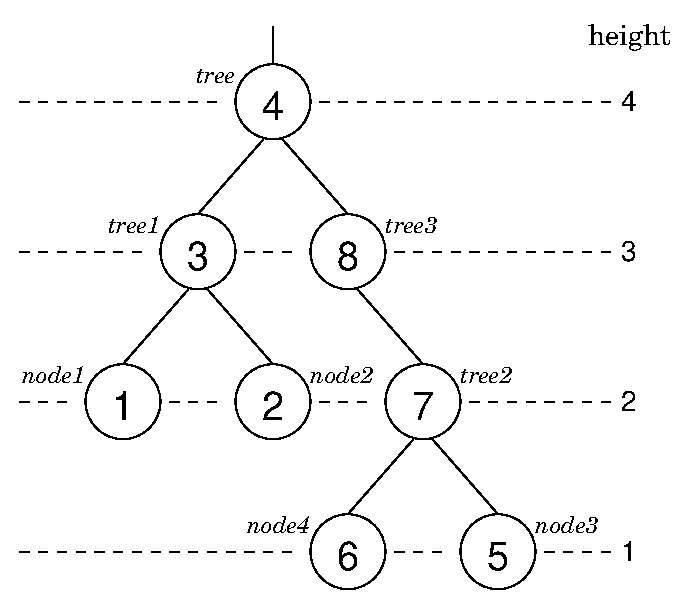
\includegraphics[height=60.0mm]{tree.eps}
\end{center}
\end{screen}

% \begin{screen}
%   \noindent\textbf{$B!Z2rEzNc(B 8$B![(B}
%   \small
% \begin{verbatim}
% int heigthTree(struct node *tree)
% {
%   int heigth = 0;
%   int leftHeigth = 0;
%   int rightHeigth = 0;


%   if (tree != (struct node*)NULL) {
%     if (tree->left != (struct node*)NULL) {
%       leftHeigth = heigthTree(tree->left);
%     }

%     if (tree->right != (struct node*)NULL) {
%       rightHeigth = heigthTree(tree->right);
%     }

%     if (leftHeigth > rightHeigth) {
%       heigth = leftHeigth + 1;
%     } else {
%       heigth = lightHeigth + 1;
%     }
%   }

%   return heigth;
% }
% \end{verbatim}
% \end{screen}


\begin{exercise}
  $B0z?t$H$7$F$"$k%G!<%?$H@aE@$X$N%]%$%s%?$r$H$j!"$=$N@aE@$r:,$H$9$kFsJ,(B
  $BLZ!JItJ,LZ!KCf$KB8:_$9$k!"$=$N%G!<%?$HF1$8CM$r$b$D@aE@$X$N%]%$%s%?$r(B
  $BJV$9:F5"4X?t(B
\begin{quote}
 \texttt{struct node *locateNode(int, struct node*);}
\end{quote}
  $B$r(B
  $B:n@.$;$h!#(B
  $B$?$@$7!"3:Ev$9$k@aE@$,$J$$>l9g$K$O(B \texttt{NULL} $B$rJV$9$3$H!#(B
  $B$J$*!"3:Ev$9$k@aE@$,J#?tB8:_$9$k>l9g$G$"$C$F$b:G=i$K8+$D$+$C$?$b$N$N(B
  $B$_$rJV$;$P$h$$!#(B
\end{exercise}

% \begin{screen}
%   \noindent\textbf{$B!Z2rEzNc(B 9$B![(B}
%   \small
% \begin{verbatim}
% struct node *locateNode(int data, struct node *tree)
% {
%   struct node *node;  /* pointer to the node */


%   if (tree == (struct node*)NULL) {
%     return (struct node*)NULL;
%   }

%   if (tree->data == data) {
%     return tree;
%   }

%   if (tree->left != (struct node*)NULL) {
%     node = locateNode(data, tree->left);
%     if (node != (struct node*)NULL) {
%       return node;
%     }
%   }

%   if (tree->right != (struct node*)NULL) {
%     node = locateNode(data, tree->right);
%     if (node != (struct node*)NULL) {
%       return node;
%     }
%   }

%   return (struct node*)NULL;
% }
% \end{verbatim}
% \end{screen}


\begin{exercise}
  $B0z?t$H$7$F@aE@$X$N%]%$%s%?$r$H$j!"$=$N@aE@$r:,$H$9$kFsJ,LZ!JItJ,LZ!K(B
  $B$r:o=|$9$k:F5"4X?t(B
\begin{quote}
 \texttt{void deleteTree(struct node*);}
\end{quote}
  $B$r:n@.$;(B
  $B$h!#(B

  \textbf{$B;29M(B)}
  $BFsJ,LZ$N:o=|$O!"$=$NFsJ,LZ$r9=@.$9$kA4$F$N@aE@$r:F5"E*$K:o=|$9$k$3$H(B
  $B$G<B8=$G$-$k$,!":o=|$9$k=gHV$KCm0U$9$k$3$H!#(B
\end{exercise}

% \begin{screen}
%   \noindent\textbf{$B!Z2rEzNc(B 10$B![(B}
% \begin{verbatim}
% void deleteTree(struct node *tree)
% {
%   if (tree != (struct node*)NULL) {
%     /* delete left sub-tree */
%     if (tree->left != (struct node*)NULL) {
%       deleteTree(tree->left);
%     }

%     /* delete right sub-tree */
%     if (tree->right != (struct node*)NULL) {
%       deleteTree(tree->right);
%     }

%     /* delete corrent node */
%     free(tree);
%   }
% }
% \end{verbatim}
% \end{screen}

\begin{exercise}
 $B<BAu$7$?FsJ,LZ$NA`:n4X?t$,@5$7$/F0:n$9$k$+3N$+$a$k$h$&$K(B\texttt{main()}
 $B4X?t$r:n@.$7!"@5$7$/F0:n$7$F$$$k$3$H$r3N$+$a$h!#(B
\end{exercise}

% \section*{$BFsJ,LZA`:n%W%m%0%i%`Nc(B}
% \label{ExampleMain}

% \begin{screen}
%   \noindent\textbf{$B!Z%W%m%0%i%`Nc![(B}
%   \scriptsize
% \begin{verbatim}
% int main(void)
% {
%   struct node *tree;
%   struct node *tree1, *tree2, *tree3;
%   struct node *node1, *node2, *node3, *node4;


%   node1 = createNode(1, (struct node*)NULL, (struct node*)NULL);
%   node2 = createNode(2, (struct node*)NULL, (struct node*)NULL);
%   tree1 = createNode(3, node1, node2);

%   node3 = createNode(5, (struct node*)NULL, (struct node*)NULL);
%   node4 = createNode(6, (struct node*)NULL, (struct node*)NULL);
%   tree2 = createNode(7, node4, node3);

%   tree3 = createNode(8, (struct node*)NULL, tree2);

%   tree = createNode(4, tree1, tree3);

%   printf("postOrder(tree): ");
%   postOrder(tree);
%   printf("\ninOrder(tree):   ");
%   inOrder(tree);
%   printf("\npreOrder(tree):  ");
%   preOrder(tree);
%   putc('\n', stdout);

%   printf("labelNode(leftNode(tree))  = %d\n", labelNode(leftNode(tree)));
%   printf("labelNode(rightNode(tree)) = %d\n", labelNode(rightNode(tree)));

%   printf("heigthTree(tree) = %d\n", heigthTree(tree));
%   printf("labelNode(locateNode(2,tree)) = %d\n", labelNode(locateNode(2, tree)));

%   deleteTree(tree);

%   return 0;
% }
% \end{verbatim}
% \end{screen}

% \begin{screen}
%   \noindent\textbf{$B!Z<B9TNc![(B}
%   \scriptsize
% \begin{verbatim}
% postOrder(): 1, 2, 3, 6, 5, 7, 8, 4, 
% inOrder():   1, 3, 2, 4, 8, 6, 7, 5, 
% preOrder():  4, 3, 1, 2, 8, 7, 6, 5, 
% leftNode  = 3
% rightNode = 8
% heigthTree = 4
% labelNode(locateNode(2)) = 2
% \end{verbatim}
% \end{screen}

% \begin{center}
% \end{center}
